\documentclass[../../main/main.tex]{subfiles}
\graphicspath{{./figures/}}

\dominitoc
\faketableofcontents

% \renewcommand{\mtcSfont}{\small\bfseries}
% \renewcommand{\mtcSSfont}{\footnotesize}

\makeatletter
\renewcommand{\@chapapp}{Chimie -- chapitre}
\makeatother

% \toggletrue{student}
% \toggletrue{corrige}
% \renewcommand{\mycol}{black}
% \renewcommand{\mycol}{gray}

\hfuzz=5.002pt

\begin{document}
\setcounter{chapter}{3}

\settype{prof}
\settype{stud}
\settype{book}

\chapter{R\'eactions acido-basiques}

\vspace*{\fill}

\begin{prgm}
	% \footnotesize
	\begin{tcb}*(ror)"know"{Savoirs}
		\begin{itemize}
			\item Constante d'acidité, diagramme de prédominance et de distribution~;
			\item Exemples usuels d'acides et bases : nom, formule et nature --
			      faible ou forte -- des acides sulfurique, nitrique, chlorhydrique,
			      phosphorique, acétique, de la sourde, l'ion hydrogénocarbonate,
			      l'ammoniac.
		\end{itemize}
	\end{tcb}
	\begin{tcb}*(ror)"how"{Savoir-faire}
		\begin{itemize}
			\item Identifier le caractère acido-basique d'une réaction en solution
			      aqueuse.
			\item Écrire l'équation de la réaction modélisant une transformation en
			      solution aqueuse en tenant compte des caractéristiques du milieu
			      réactionnel (nature des espèces chimique en présence, pH…) et des
			      observations expérimentales.
		\end{itemize}
	\end{tcb}
\end{prgm}

\vspace*{\fill}
\minitoc
\vspace*{\fill}

\newpage

\vspace*{\fill}
% {
\begin{boxes}
	% \footnotesize
	\begin{tcb}(defi)<lftt>{Liste des définitions}
		\tcblistof[\paragraph*]{defi}{\hspace*{6pt}}
	\end{tcb}
	% \begin{tcb}(rapp)<lftt>{Liste des rappels}
	% 	\tcblistof[\paragraph*]{rapp}{\hspace*{6pt}}
	% \end{tcb}
	\begin{tcb}(prop)<lftt>{Liste des propriétés}
		\tcblistof[\paragraph*]{prop}{\hspace*{6pt}}
		% \tcblistof[\paragraph*]{loi}{\hspace*{6pt}}
		\tcblistof[\paragraph*]{theo}{\hspace*{6pt}}
	\end{tcb}
	% \begin{tcb}(coro)<lftt>{Liste des corollaires}
	% 	\tcblistof[\paragraph*]{coro}{\hspace*{6pt}}
	% \end{tcb}
	\begin{tcb}(demo)<lftt>{Liste des démonstrations}
		\tcblistof[\paragraph*]{demo}{\hspace*{6pt}}
		\tcblistof[\paragraph*]{prev}{\hspace*{6pt}}
	\end{tcb}
	\begin{tcb}(inte)<lftt>{Liste des interprétations}
		\tcblistof[\paragraph*]{inte}{\hspace*{6pt}}
	\end{tcb}
	% \begin{tcb}(tool)<lftt>{Liste des outils}
	% 	\tcblistof[\paragraph*]{tool}{\hspace*{6pt}}
	% \end{tcb}
	% \begin{tcb}(nota)<lftt>{Liste des notations}
	% 	\tcblistof[\paragraph*]{nota}{\hspace*{6pt}}
	% \end{tcb}
	\begin{tcb}(appl)<lftt>{Liste des applications}
		\tcblistof[\paragraph*]{appl}{\hspace*{6pt}}
	\end{tcb}
	\begin{tcb}(rema)<lftt>{Liste des remarques}
		\tcblistof[\paragraph*]{rema}{\hspace*{6pt}}
	\end{tcb}
	\begin{tcb}(exem)<lftt>{Liste des exemples}
		\tcblistof[\paragraph*]{exem}{\hspace*{6pt}}
	\end{tcb}
	\begin{tcb}(ror)<lftt>{Liste des points importants}
		\tcblistof[\paragraph*]{ror}{\hspace*{6pt}}
	\end{tcb}
	\begin{tcb}(impo)<lftt>{Liste des erreurs communes}
		\tcblistof[\paragraph*]{impo}{\hspace*{6pt}}
	\end{tcb}
\end{boxes}
% }
\vspace*{\fill}
\newpage

\section{Acides et bases}
\subsection{Couples acido-basiques}
\begin{tcb*}(defi){Acides et bases}
	\begin{itemize}
		\bitem{Un acide} est une espèce chimique capable de \textbf{céder} un proton
		\ce{H+}.
		\bitem{Une base} est une espèce chimique capable de \textbf{capter} un
		proton \ce{H+}.
		\bitem{Un couple acido-basique} est la donnée d'un acide et de sa base
		\textbf{conjuguée} (espèce obtenu quand l'acide a donné son proton)
		\bitem{Un polyacide} est une espèce qui peut céder plusieurs protons~;
		de même pour une \textbf{polybase} qui peut en capter plusieurs.
		\bitem{Une espèce amphotère} est une espèce qui peut se trouver à la fois
		acide d'un couple mais base d'un autre. On dit que c'est un
		\textbf{ampholyte}.
	\end{itemize}
\end{tcb*}

\begin{tcb*}*[sidebyside](exem)<lftt>"ror"{Couples à connaître}
	\begin{itemize}
		\item Oxonium/eau
		      \begin{center}
			      \psw[red]{\ce{H3O+}}/\psw[blue]{\ce{H2O}}
		      \end{center}
		\item Acide chlorhydrique/ion chlorure
		      \begin{center}
			      \psw[red]{\ce{HCl}}/\psw[blue]{\ce{Cl-}}
		      \end{center}
		\item Acide sulfurique/ion hydrogénosulfate
		      \begin{center}
			      \psw[red]{\ce{H2SO4}}/\psw[blue]{\ce{HSO4-}}
		      \end{center}
		\item Ion hydrogénosulfate/ion sulfate
		      \begin{center}
			      \psw[red]{\ce{HSO4-}}/\psw[blue]{\ce{SO4^2-}}
		      \end{center}
		\item Acide phosphorique (triacide)
		      \begin{center}
			      \psw[red]{\ce{H3PO4}}/\psw{\ce{H2SO4^{2-}}}/\psw{\ce{HPO4^{2-}}}/\psw[blue]{\ce{PO4^{3-}}}
		      \end{center}
	\end{itemize}
	\tcblower
	\begin{itemize}
		\item Acide nitrique/ion nitrate
		      \begin{center}
			      \psw[red]{\ce{HNO4}}/\psw[blue]{\ce{NO3^-}}
		      \end{center}
		\item Acide éthanoïque/ion éthanoate
		      \begin{center}
			      \psw[red]{\ce{CH3COOH}}/\psw[blue]{\ce{CH3COO-}}
		      \end{center}
		\item Acide carbonique/ion hydrogénocarbonate
		      \begin{center}
			      \psw[red]{\ce{H2CO3}}/\psw[blue]{\ce{HCO3-}}
		      \end{center}
		\item Ion ammonium/ammoniac
		      \begin{center}
			      \psw[red]{\ce{NH4+}}/\psw[blue]{\ce{NH3}}
		      \end{center}
		\item Eau/ion hydroxyde
		      \begin{center}
			      \psw[red]{\ce{H2O}}/\psw[blue]{\ce{HO-}}
		      \end{center}
	\end{itemize}
\end{tcb*}

\begin{tcb*}(rema)<lftt>{Solvant et écriture générique}
	\begin{itemize}
		\item Tous ces ions ne peuvent exister quand dans un solvant adapté. En pratique,
		      \textbf{on se placera toujours dans l'eau}.
		\item Pour une écriture générique, on écrira un couple
		      \begin{center}
			      \ce{AH}/\ce{A-}
		      \end{center}
		      même si parfois c'est l'acide qui est chargé positivement et la base
		      neutre (\ce{NH4+}/\ce{NH3}). C'est une notation de commodité.
	\end{itemize}
\end{tcb*}

Ainsi, un acide dans un milieu aura tendance à libérer des ions \ce{H+}.
Seulement, ces ions n'existent pas dans l'eau de manière stable~: il sera
forcément capté par une autre base, et à défaut par l'eau. On peut donc mesurer
l'acidité d'une solution en mesurant la concentration $[\ce{H_3O+}]$.

\subsection{Le pH}
\begin{tcb*}(defi){pH}
	Le pH d'une \textbf{solution aqueuse} est
	\psw{
		\[
			\pH = - \log (\frac{[\ce{H_3O+}]}{c^\circ})
			\Lra
			[\ce{H_3O+}] = c^\circ10^{-\pH}
		\]
	}
	\vspace{-15pt}
	\begin{itemize}
		\bitem{Un pH faible} correspond à une solution \psw{\textbf{acide}}
		\bitem{Un pH élevée} correspond à une solution \psw{\textbf{basique}}
	\end{itemize}
\end{tcb*}
\begin{tcb*}(rema)<lftt>{Opérateur p}
	Le «~p~» de pH est en fait un raccourci pour une opération. Pour une grandeur
	\textbf{adimensionnée} $X$, on définit
	\[
		\prm X = - \log X
	\]
\end{tcb*}
\begin{tcb*}(exem)<lftt>{pH et concentration}
	% \vspace{-15pt}
	$\begin{array}{ll}
			\diamond~\pH = 3                             & \Ra [\ce{H3O+}] = \psw{\SI{e-3}{mol.L^{-1}}}
			\\
			\diamond~[\ce{H_3O+}] = \SI{e-5}{mol.L^{-1}} & \Ra \pH = \psw{5}
		\end{array}$
\end{tcb*}

\section{Réactions acido-basiques en solution}
\subsection{Constante d'acidité}
\begin{tcb*}(defi){Constante d'acidité}
	Pour un couple \ce{AH}/\ce{A-}, la constante d'équilibre associée est celle de
	\textbf{l'acide avec l'eau}~:
	\psw{
		\begin{gather*}
			\psw[red]{\ce{AH\aqu{}}} + \psw[blue]{\ce{H_2O\liq{}}} \ce{=}
			\psw[blue]{\ce{A^-\aqu{}}} + \psw[red]{\ce{H_3O+\aqu{}}}
			\tag*{$K_A$}
			\\\beforetext{D'où}
			\boxed{
				K_A =
				\frac{[\ce{H_3O+}]\ind{eq}\times [\ce{A-}]\ind{eq}}{[\ce{AH}]\ind{eq}c^\circ}
			}
		\end{gather*}
	}
	On aura alors $\pk = - \log K_A$ qui sont les données tabulées et
	données.
\end{tcb*}
\begin{tcb*}(exem)<lftt>{Constantes d'acidités}
	On donne des $\pk$, donner les $K_A$~:
	\[
		\pk(\ce{CH_3COOH/CH_3COO-}) = \num{4.75}
		\qet
		\pk(\ce{NH_4+/NH_3}) = \num{9.2}
	\]
	\tcblower
	\psw{
		\[
			K_A(\ce{CH_3COOH/CH_3COO-}) = 10^{-\num{4.75}}
			\qet
			K_A(\ce{NH_4+/NH_3}) = 10^{-\num{9.2}}
		\]
	}
	\vspace{-15pt}
\end{tcb*}

\begin{tcb*}[breakable](appl)<lftt>{Calcul direct d'un $K_A$}
	On mélange une solution d'acide éthanoïque à $c_0 = \SI{e-2}{mol.L^{-1}}$ dans
	de l'eau, et on mesure $[\ce{H_3O+}]\ind{eq} =
		10^{-\num{3.38}}\si{mol.L^{-1}}$. Dresser le tableau d'avancement, déterminer
	l'état final puis déterminer la valeur de $K_A$ du couple.
	\tcblower
	\begin{center}
		\def\rhgt{0.50}
		\centering
		\begin{tabularx}{\linewidth}{|l|c||YdYdYdY|}
			\hline
			\multicolumn{2}{|c||}{
				$\xmathstrut{\rhgt}$
			\textbf{Équation}}         &
			\psw{$\ce{CH_3COOH\aqu}$}  & $+$                    &
			\psw{$\ce{H_2O\liq}$}      & $\ra$                  &
			\psw{$\ce{CH_3COO^-\aqu}$} & $+$                    &
			\psw{$\ce{H_3O^+\aqu}$}                               \\
			\hline
			$\xmathstrut{\rhgt}$
			Initial                    & $x = 0$                &
			\psw{$c_0$}                & \vline                 &
			\psw{excès}                & \vline                 &
			\psw{$0$}                  & \vline                 &
			\psw{$0$}                                             \\
			\hline
			$\xmathstrut{\rhgt}$
			Final                      & $x_f = \psw{x_{\equ}}$ &
			\psw{$c_0 - x_{\equ}$}     & \vline                 &
			\psw{excès}                & \vline                 &
			\psw{$x_{\equ}$}           & \vline                 &
			\psw{$x_{\equ}$}                                      \\
			\hline
		\end{tabularx}
	\end{center}
	\vspace{-15pt}
	\psw{
		\begin{gather*}
			x\ind{max} = c_0
			\qet
			[\ce{H_3O+}]_f = x_f < x\ind{max}
			\quad \text{donc équilibre}
			\\\Ra
			\boxed{x_f = x\ind{eq} = 10^{\num{-3.38}}\si{mol.L^{-1}}}
			\\\beforetext{Ainsi}
			\boxed{K_A = \frac{x\ind{eq}^2}{c_0-x\ind{eq}}}
			\Ra
			\xul{K_A = \num{1.8e-5} = 10^{-\num{4.74}}}
			\qed
		\end{gather*}
	}
	\vspace{-15pt}
\end{tcb*}

\subsection{Cas particulier de l'eau}

En tant qu'ampholyte, l'eau intervient dans deux couples~:
\begin{gather*}
	\psw[red]{\ce{H3O+}}/\psw[blue]{\ce{H2O}}
	\qet
	\psw[red]{\ce{H2O}}/\psw[blue]{\ce{HO-}}
	\\
	\beforetext{Le premier couple donne}
	\psw[red]{\ce{H_3O+}} \psw{\ce{+}} \psw[blue]{\ce{H_2O}} \psw{\ce{=}}
	\psw[blue]{\ce{H_2O}} \psw{\ce{+}} \psw[red]{\ce{H_3O+}}
	\tag*{$K^\circ = \psw{1}$}
\end{gather*}
Le second donne une réaction remarquable~:

\begin{tcb*}(prop){Autoprotolyse de l'eau}
	La réaction d'autoprotolyse de l'eau est la réaction de \textbf{l'eau sur
		elle-même}, et sa constante est appelée \textbf{produit ionique de l'eau}
	noté $K_e$~:
	\begin{gather*}
		\psw{2 \ce{H_2O}} =
		\psw[red]{\ce{H_3O+}} \psw{+}
		\psw[blue]{\ce{HO-}}
		\tag*{$K_e(\SI{25}{\degreeCelsius}) = \psw{\num{e-14}}$}
		\\\beforetext{Avec donc}
		\boxed{
			\psw{K_e = \frac{[\ce{H_3O+}]\ind{eq}\times [\ce{HO-}]\ind{eq}}{{c^\circ}^2}}
		}
	\end{gather*}
\end{tcb*}
\begin{tcb*}(inte){Autoprotolyse de l'eau}
	Ainsi, dans de l'eau pure, il y aura forcément des ions oxonium et hydroxyde,
	mais surtout en solution aqueuse la quantité d'ions \ce{H3O+} est directement
	reliée à celle des ions \ce{HO-}~: \textbf{l'un n'évolue pas sans l'autre}.
\end{tcb*}

\begin{tcb*}[breakable](appl)<lftt>{pH de l'eau pure}
	Déterminer donc le pH de l'eau pure.
	\tcblower
	\psw{
		\begin{center}
			\def\rhgt{0.35}
			\centering
			\begin{tabularx}{\linewidth}{|l|c||YdYdY|}
				\hline
				\multicolumn{2}{|c||}{
					$\xmathstrut{\rhgt}$
				\textbf{Équation}} &
				$\ce{H_2O\liq}$    & $+$              &
				$\ce{H_3O+\aqu}$   & $+$              &
				$\ce{HO^-\aqu}$                         \\
				\hline
				$\xmathstrut{\rhgt}$
				Initial            & $x = 0$          &
				excès              & \vline           &
				$0$                & \vline           &
				$0$                                     \\
				\hline
				$\xmathstrut{\rhgt}$
				Final              & $x_f = x_{\equ}$ &
				excès              & \vline           &
				$x_{\equ}$         & \vline           &
				$x_{\equ}$                              \\
				\hline
			\end{tabularx}
		\end{center}
		\vspace{-15pt}
		\begin{gather*}
			\beforetext{Ainsi}
			[\ce{H_3O+}]\ind{eq} = x\ind{eq}
			\qet
			K_e = \left( \frac{x\ind{eq}}{c^\circ} \right)^2
			\Lra
			\frac{[\ce{H_3O+}]\ind{eq}}{c^\circ} = c^\circ \sqrt{K_e}
			\\\Lra
			\pH = \frac{1}{2}\pk[e]
			\Lra
			\boxed{\pH = 7}
		\end{gather*}
		On dit que l'eau est \textbf{neutre}.
	}
\end{tcb*}

\subsection{Réaction entre couples}
\begin{tcb*}[sidebyside, righthand ratio=.4](defi){Réaction acide-base}
	Une réaction entre un acide \ce{AH} et une base \ce{B-} est l'action de
	l'acide d'un couple avec la base d'un autre, et résulte en l'échange d'un (ou
	plusieurs) protons~:
	\[
		\psw[red]{\ce{AH}} + \psw[blue]{\ce{B-}} \ce{=}
		\psw[blue]{\ce{A-}} + \psw[red]{\ce{BH}}
	\]
	\tcblower
	\begin{center}
		\includegraphics[width=\linewidth]{ab_echH}
	\end{center}
\end{tcb*}

Comme dans les chapitres précédents, on va souvent s'intéresser à des calculs de
constantes de réaction, il y aura deux manières de procéder. Prenons un
exemple~:
\begin{tcb*}[breakable](appl)<lftt>{Calcul de constantes de réactions}
	Soit la réaction entre l'ion éthanoate et l'ion ammonium~:
	\begin{gather*}
		\beforetext{$K^\circ$}
		\red{\ce{CH_3COO^-\aqu}} + \blu{\ce{NH_4^+\aqu}}
		=
		\red{\ce{CH_3COOH\aqu}} + \blu{\ce{NH_3\aqu}}
		\tag{R}
		\label{eq:R}
		\\
		\pk(\ce{NH_4+/NH_3}) = \pk[A,1] = \num{9.2}
		\qet
		\pk(\ce{CH_3COOH/CH_3COO-}) = \pk[A,2] = \num{4.75}
	\end{gather*}
	\begin{enumerate}[label=\sqenumi]
		\item Déterminer la constante de réaction en exprimant $K^\circ$, $K_{A,1}$
		      et $K_{A,2}$ et en les combinant.
		\item Déterminer la constante de réaction en trouvant un lien entre les 3
		      équations.
	\end{enumerate}
	\tcblower
	\begin{enumerate}[label=\sqenumi]
		\mitem \psw{
			\begin{gather*}
				K_{A,1} = \frac{[\ce{H_3O+}]\ind{eq}\times
					[\ce{NH_3}]\ind{eq}}{[\ce{NH_4+}]\ind{eq}}
				\qet
				K_{A,2} = \frac{[\ce{H_3O+}]\ind{eq}\times
					[\ce{CH_3COO-}]\ind{eq}}{[\ce{CH_3COOH}]\ind{eq}}
				\\\beforetext{Or}
				K = \frac{[\ce{CH_3COOH}]\ind{eq}\times [\ce{NH_3}]\ind{eq}}
				{[\ce{CH_3COO-}]\ind{eq}\times [\ce{NH_4+}]\ind{eq}} \times
				\underbracket[1pt]{\frac{[\ce{H_3O+}]\ind{eq}}{[\ce{H_3O+}]\ind{eq}}}_{=1}
				\\\beforetext{On identifie}
				\boxed{K^\circ = \frac{K_{A,1}}{K_{A,2}}}
				\Ra
				\xul{K^\circ = 10^{\num{-4.45}}}
			\end{gather*}
		}
		\mitem \psw{
			\begin{align*}
				\beforetext{$K_{A,1}$}
				\psw[red]{\ce{NH_4^+\aqu}} + \psw[blue]{\ce{H_2O\liq}}   & =
				\psw[blue]{\ce{NH_3\aqu}} + \psw[red]{\ce{H_3O+\aqu}}
				\tag{1}
				\label{eq:1}
				\\
				\beforetext{$K_{A,2}$}
				\psw[red]{\ce{CH_3COOH\aqu}} + \psw[blue]{\ce{H_2O\liq}} & =
				\psw[blue]{\ce{CH_3COO^-\aqu}} + \psw[red]{\ce{H_3O+\aqu}}
				\tag{2}
				\label{eq:2}
				\\
				\eqref*{eq:R} = \eqref*{eq:1} - \eqref*{eq:2}
				                                                         & \Ra
				\boxed{K^\circ = \frac{K_{A,1}}{K_{A,2}}}
			\end{align*}
		}
		\vspace{-15pt}
	\end{enumerate}
\end{tcb*}

\section{Distribution des espèces d'un couple}
\subsection{Relation entre pH et concentrations}
\begin{tcb*}(prop){Relation de \textsc{Henderson}}
	Pour un unique couple acide-base en solution, on a la relation suivante~:
	\psw{
		\[
			\boxed{\pH = \pk + \log \frac{[\ce{A-}]}{[\ce{AH}]}}
		\]
	}
\end{tcb*}
\begin{tcb*}(demo)<lftt>{Relation de \textsc{Henderson}}
	\psw{
		\begin{DispWithArrows*}
			K_A \triangleq
			\frac{[\ce{H_3O+}]\ind{eq}\times [\ce{A-}]\ind{eq}}{[\ce{AH}]\ind{eq}c^\circ}
			&\Lra
			\frac{[\ce{H_3O+}]\ind{eq}}{c^\circ} =
			K_A\frac{[\ce{AH}]\ind{eq}}{[\ce{A-}]\ind{eq}}
			\CArrow{$-\log \cdot $}
			\\
			-\log [\ce{H_3O+}]\ind{eq} =
			-\log K_A - \log \frac{[\ce{AH}]\ind{eq}}{[\ce{A-}]\ind{eq}}
			& \Lra
			\boxed{\pH = \pk + \log \frac{[\ce{A-}]}{[\ce{AH}]}}
			\qed
		\end{DispWithArrows*}
	}
	\vspace{-15pt}
\end{tcb*}
\begin{tcb}(rema)<lftt>{Remarque}
	On retrouve bien que le pH augmente lorsque l'on ajoute de la base, et
	inversement.
\end{tcb}

\subsection{Diagramme de prédominance}
\begin{tcb*}(ror){Diagramme de prédominance}
	D'après la formule précédente, on remarque que
	\begin{itemize}
		\item \psw{
		      $[\ce{AH}] = [\ce{A-}] \Ra \pH = \pk$
		      }
		\item \psw{
			      $[\ce{AH}] > [\ce{A-}] \Ra \pH > \pk$~; on dit que \textbf{l'acide
				      prédomine}
		      }
		\item \psw{
		      $[\ce{AH}] = [\ce{A-}] \Ra \pH = \pk$~; on dit que \textbf{la base
			      prédomine}
		      }
	\end{itemize}
	De plus, on peut trouver quand est-ce qu'une espèce est majoritaire, i.e.\ sa
	concentration est 10 fois supérieure à celle de l'espèce conjuguée~:
	\begin{itemize}
		\item \psw{
			      $[\ce{AH}] > 10[\ce{A-}] \Ra \pH < \pk - 1$~; on dit que \textbf{l'acide
				      est majoritaire}
		      }
		\item \psw{
			      $[\ce{A-}] > 10[\ce{AH}] \Ra \pH > \pk + 1$~; on dit que \textbf{la
				      base est majoritaire}
		      }
	\end{itemize}
	On trace ainsi le \textbf{diagramme de prédominance} d'un couple
	acido-basique~:
	\begin{center}
		\sswitch{
			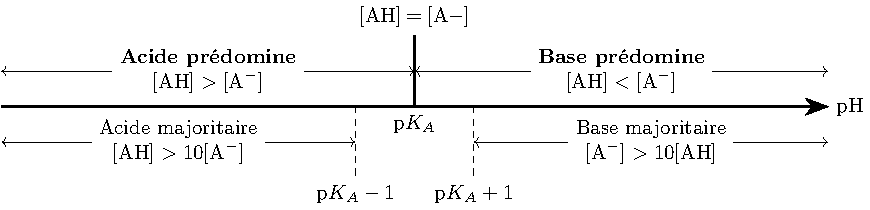
\includegraphics[scale=1, draft=true]{predom.pdf}
		}{
			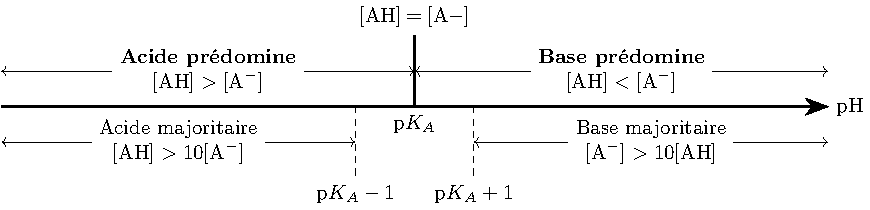
\includegraphics[scale=1]{predom.pdf}
		}
		\captionof{figure}{Diagramme de prédominance générique}
	\end{center}
\end{tcb*}

\begin{tcb*}(inte){Diagramme combiné~: réaction spontanée}
	Les diagrammes de prédominances permettent de savoir si deux espèces
	réagissent. En effet, deux espèces qui ont des domaines de prédominance
	disjoints vont réagir ensemble pour donner les espèces qui peuvent exister
	ensemble au même pH. Il suffit donc de tracer un diagramme avec les
	différents couples pour trouver la réaction spontanée~:
	\begin{center}
		\sswitch{
			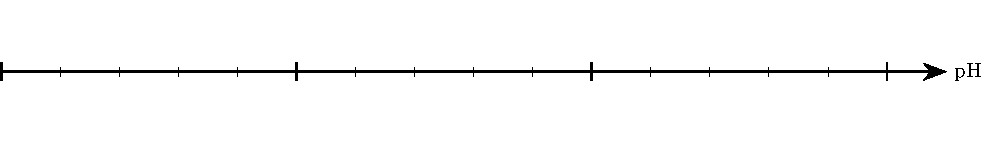
\includegraphics[scale=1]{predom_2-plain}
		}{
			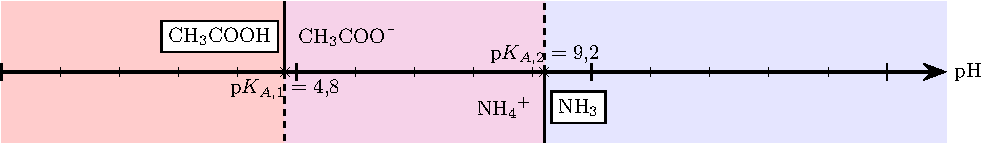
\includegraphics[scale=1]{predom_2}
		}
	\end{center}
\end{tcb*}

\begin{tcb*}(defi){Indicateur coloré}
	Un indicateur coloré est une espèce chimique dont les formes acide et basique
	n'ont pas la même couleur. La \textbf{zone de virage} est la zone de pH où les
	deux formes sont présentes, et que l'indicateur a une couleur intermédiaire.
\end{tcb*}
\begin{tcb*}(exem)<lftt>{Indicateurs colorés}
	\begin{itemize}
		\item Le bleu de bromothymol (BBT)~: $\pk = \num{7.3}$
		\item La phénolphtaléine~: $\pk = \num{9.4}$
	\end{itemize}
	Le papier pH repose sur ce principe, en utilisant plusieurs indicateurs
	colorés.
\end{tcb*}

\begin{tcb*}[sidebyside, righthand ratio=.25](defi){Force des acides et des bases}
	\begin{itemize}
		\bitem{Un acide fort} est un acide qui se \textbf{dissout totalement} dans
		l'eau. Son $\pk$ est alors \xul{\psw{petit}}, et sa base conjuguée est dite
		faible.
		\psw{
			\begin{gather*}
				\psw[red]{\ce{AH}} \ce{+} \psw[blue]{\ce{H_2O}} \ce{->}
				\psw[blue]{\ce{A-}} \ce{+} \psw[red]{\ce{H_3O+}}
				\tag*{$K_A \gg 1 \Lra \pk \leq 0$}
			\end{gather*}
		}
		\vspace{-15pt}
		\bitem{Une base forte} est une base qui se \textbf{dissout totalement} dans
		l'eau. Son $\pk$ est alors \xul{\psw{grand}}, et son acide conjugué est dit
		faible.
		\psw{
			\begin{gather*}
				\psw[red]{\ce{AH}} \ce{+} \psw[blue]{\ce{H_2O}} \ce{<-}
				\psw[blue]{\ce{A-}} \ce{+} \psw[red]{\ce{H_3O+}}
				\tag*{$K_A \ll 1 \Lra \pk \geq 14$}
			\end{gather*}
		}
		\vspace{-15pt}
	\end{itemize}
	On peut alors les classer grâce à une échelle de $\pk$~:
	\tcblower
	\begin{center}
		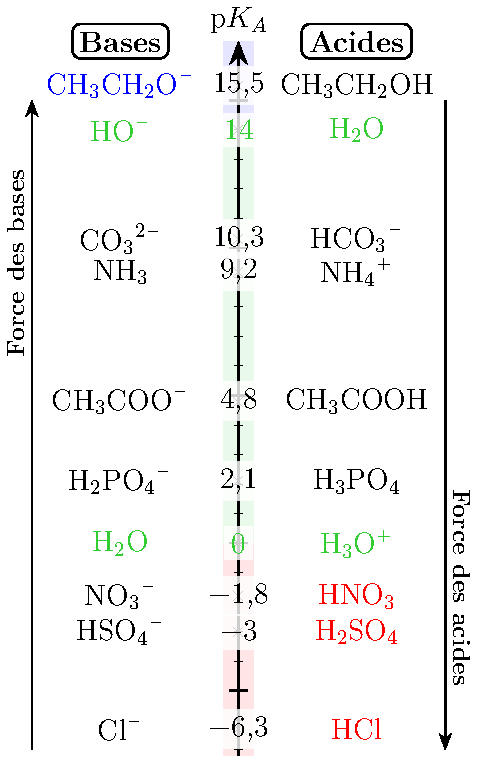
\includegraphics[width=\linewidth]{pka_scale}
		\captionsetup{justification=centering}
		\captionof{figure}{\\Échelle des $\pk$}
	\end{center}
\end{tcb*}
\begin{tcb*}[cnt, bld](impo){Échelle des $\pk$ et ordre}
	Dans une échelle des $\pk$, les bases sont à gauche~!
\end{tcb*}

\subsection{Diagramme de distribution}
On peut avoir plus de détail sur la répartition en traçant la proportion de
l'acide et de la base en fonction du pH.
\begin{tcb*}[breakable](exem)<lftt>{Diagrammes de distributions}
	\begin{itemize}
		\bitem{Monoacide}~:
		En appelant $\alpha(\ce{CH_3COOH})$ la fraction en acide éthanoïque, le
		diagramme de distribution entre lui et sa base conjuguée est
		% TODO: Idem, facile à faire avec Henderson
		\begin{center}
			\sswitch{
				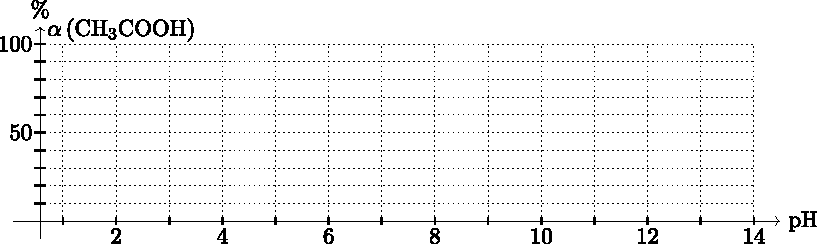
\includegraphics[scale=1]{distrib_ethan-plain}
			}{
				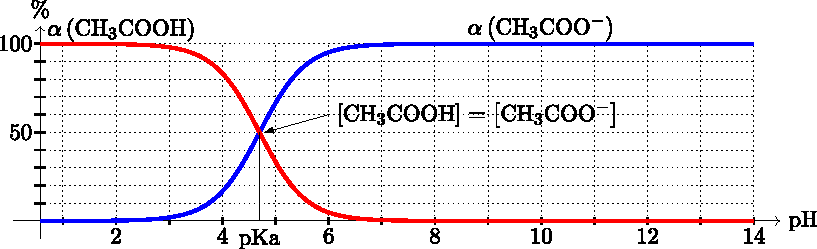
\includegraphics[scale=1]{distrib_ethan}
			}
		\end{center}
		\bitem{Polyacide}~:
		On trouve plusieurs courbes, avec les formes acides qui dominent à bas pH et
		les formes basiques à haut pH. Sur le graphique suivant, donner les formes
		basiques en solution de l'acide carbonique \ce{H2CO3}, attribuez les courbes
		aux espèces et en déduire les $\pk$.
		\begin{center}
			\sswitch{
				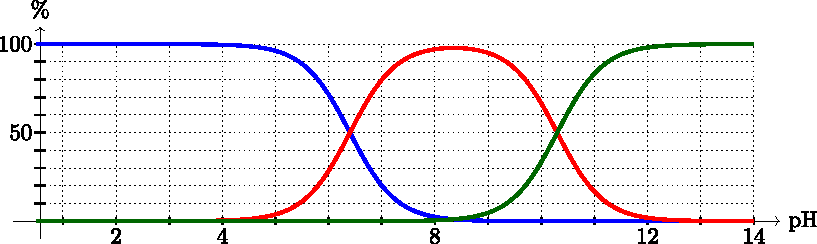
\includegraphics[scale=1]{distrib_carbo-plain}
			}{
				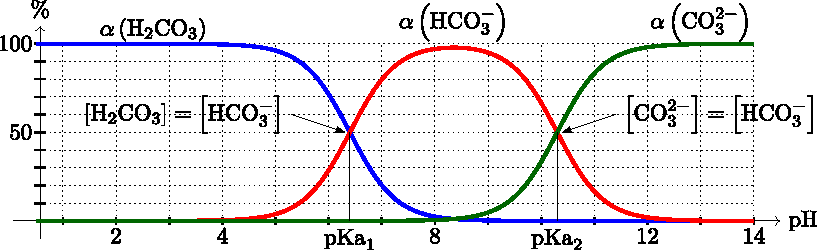
\includegraphics[scale=1]{distrib_carbo}
			}
		\end{center}
	\end{itemize}
\end{tcb*}

\section{Méthode détermination du pH d'une solution}
\begin{tcb*}(ror){Méthode de la réaction prépondérante}
	\begin{enumerate}[label=\sqenumi]
		\item Lors de la réaction entre plusieurs couples acide-base,
		      on dresse une échelle en $\pk$ en mettant les couples, et on
		      \textbf{encadre les espèces présentes}.
		\item La \textbf{réaction prépondérante} est alors celle entre
		      \textbf{l'acide présent le plus fort} et la \textbf{base présente la plus
			      forte}\ftn{On néglige \ce{HO-} et \ce{H3O+} en solution si on partait
			      avec de l'eau.}.
		\item La RP est \textbf{favorisée} selon la \textbf{règle du gamma}~:
		      \smallbreak
		      \begin{isd}
			      \begin{center}
				      \sswitch{
					      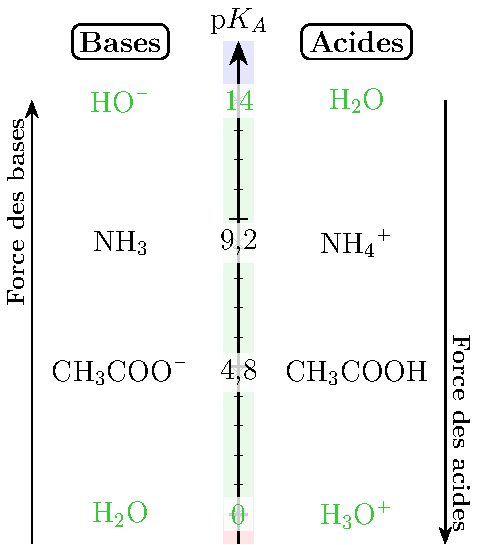
\includegraphics[width=.6\linewidth]{gamma_plain}
				      }{
					      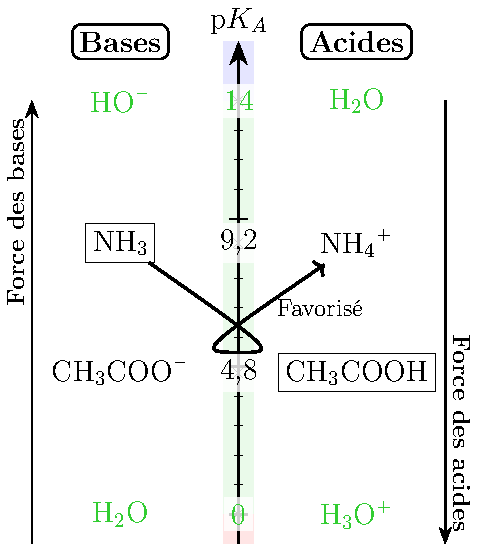
\includegraphics[width=.6\linewidth]{gamma_fav}
				      }
				      \captionof{figure}{Favorisé}
			      \end{center}
			      \tcblower
			      \begin{center}
				      \sswitch{
					      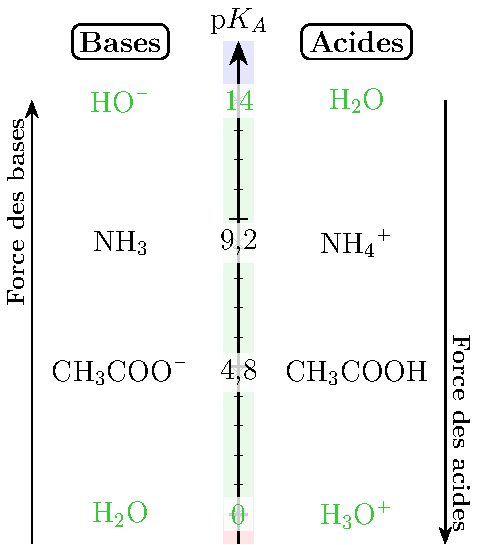
\includegraphics[width=.6\linewidth]{gamma_plain}
				      }{
					      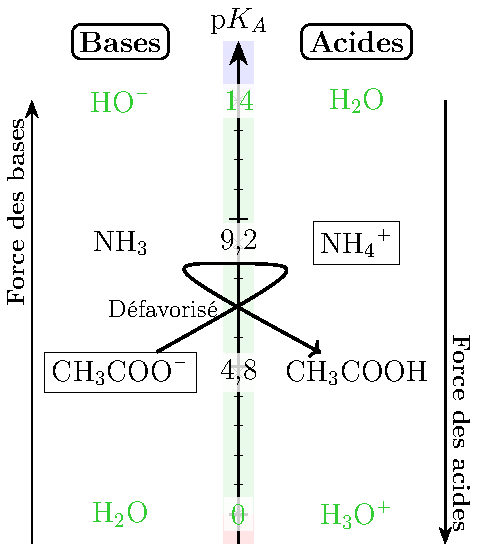
\includegraphics[width=.6\linewidth]{gamma_unfav}
				      }
				      \captionof{figure}{Défavorisé}
			      \end{center}
		      \end{isd}
		      Et on trouve la constante de la RP en calculant~:
		      \psw{
			      \[
				      K^\circ = 10^{\pk[\rm base]-\pk[\rm acide]}
				      \quad \Lra \quad
				      K^\circ = 10^{\abs{\Delta{\pk}}} \quad \text{si favorisé}
				      \qet
				      K^\circ = 10^{-\abs{\Delta{\pk}}} \quad \text{sinon}
			      \]
		      }
		      \vspace{-20pt}
		\item On dresse un tableau d'avancement et on résout, si besoin avec la
		      relation d'\textsc{Henderson}. Si la RP est totale, on recommence avec les
		      espèces restantes.
	\end{enumerate}
\end{tcb*}

\begin{tcb*}(appl)<lftt>{Détermination d'un pH à l'équilibre}
	On mélange $V_0 = \SI{50}{mL}$ d'une solution d'acide éthanoïque à
	$c_0 = \SI{0.10}{mol.L^{-1}}$, et le même volume d'une solution de nitrite de sodium
	$\left( \ce{Na+};\ce{NO_2-} \right)$ à la même concentration. On donne
	\[
		\pk[A,1] = \pk(\ce{CH_3COOH}/\ce{CH_3COO-}) = \num{4.74}
		\qet
		\pk[A,2] = \pk(\ce{HNO_2}/\ce{NO_2-}) = \num{3.2}
	\]
	\begin{center}
		\fbox{\textbf{Déterminer les concentrations des espèces à l'équilibre et le
				pH}}
	\end{center}
	\tcblower
	\noindent
	\begin{minipage}[t]{.60\linewidth}
		\begin{enumerate}[label=\sqenumi]
			\item \psw{
				      On dresse l'échelle de $\pk$ et on encadre les espèces présentes~;
			      }
			\item \psw{
				      Réaction prépondérante~:
				      \begin{gather*}
					      \ce{CH_3COOH\aqu + NO_2^-\aqu = CH_3COO^-\aqu + HNO_2\aqu}
					      \tag*{$K^\circ = 10^{\pk[A,2]-\pk[A,1]} = 10^{\num{-1.54}}$}
				      \end{gather*}
			      }
			\item \psw{
				      Elle est en effet limitée.
			      }
			\item \psw{
			      On dresse le tableau, en faisant attention au fait qu'on a dilué par
			      2~:
			      \[
				      [\ce{CH_3COOH}]_0 = \frac{c_0V_0}{V} = \frac{c_0}{2} = [\ce{NO_2^-}]
			      \]
			      }
		\end{enumerate}
	\end{minipage}
	\hfill
	\begin{minipage}[t]{.35\linewidth}
		\vspace{0pt}
		\begin{center}
			\sswitch{
				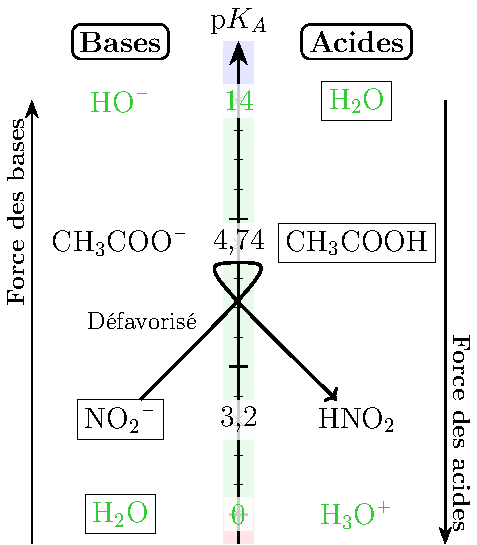
\includegraphics[width=\linewidth, draft=true]{appl_fin}
			}{
				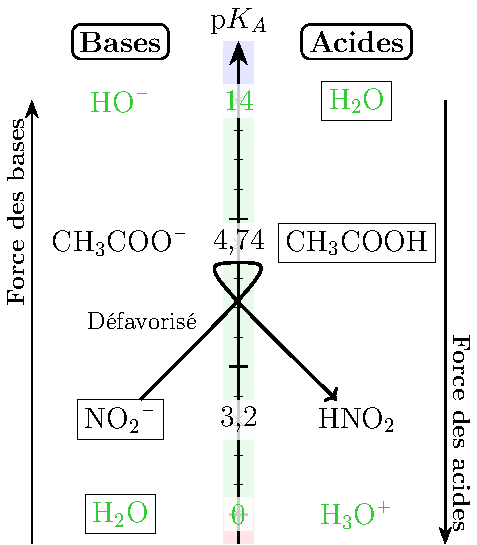
\includegraphics[width=\linewidth]{appl_fin}
			}
			\captionof{figure}{Échelle $\pk$}
		\end{center}
	\end{minipage}
	\begin{enumerate}[label=\sqenumi]
		\item[]
			\begin{center}
				\def\rhgt{0.50}
				\centering
				\begin{tabularx}{\linewidth}{|l|c||YdYdYdY|}
					\hline
					\multicolumn{2}{|c||}{
						$\xmathstrut{\rhgt}$
					\textbf{Équation}}         &
					\psw{$\ce{CH_3COOH\aqu}$}  & $+$                    &
					\psw{$\ce{NO_2^-\aqu}$}    & $=$                    &
					\psw{$\ce{CH_3COO^-\aqu}$} & $+$                    &
					\psw{$\ce{HNO_2\aqu}$}                                \\
					\hline
					$\xmathstrut{\rhgt}$
					Initial                    & $x = 0$                &
					\psw{$c_0/2$}              & \vline                 &
					\psw{$c_0/2$}              & \vline                 &
					\psw{$0$}                  & \vline                 &
					\psw{$0$}                                             \\
					\hline
					$\xmathstrut{\rhgt}$
					Final                      & $x_f = \psw{x_{\equ}}$ &
					\psw{$c_0/2 - x_{\equ}$}   & \vline                 &
					\psw{$c_0/2 - x_{\equ}$}   & \vline                 &
					\psw{$x_{\equ}$}           & \vline                 &
					\psw{$x_{\equ}$}                                      \\
					\hline
				\end{tabularx}
			\end{center}
			\psw{
				\begin{gather*}
					K^\circ = \frac{x\ind{eq}^2}{\left( c_0/2-x\ind{eq} \right)^2}
					\underbracket[1pt]{\Ra}_{x\ind{eq}>0}
					x\ind{eq} = \left( \frac{c_0}{2}-x\ind{eq} \right)\sqrt{K^\circ}
					\\\Lra
					\boxed{x\ind{eq} = \frac{\sqrt{K^\circ}}{1+\sqrt{K}}\frac{c_0}{2}}
					\Ra
					\xul{x\ind{eq} = \SI{7.3e-3}{mol.L^{-1}}}
					\\\Ra
					\left\{
					\begin{array}{rl}
						[\ce{CH_3COOH}]\ind{eq}     & = [\ce{NO_2-}]\ind{eq} = \SI{4.27e-2}{mol.L^{-1}}
						\\%
						\pac{\ce{CH_3COO-}}\ind{eq} & = [\ce{HNO_2}]\ind{eq} = \SI{7.3e-3}{mol.L^{-1}}
					\end{array}
					\right.
					\\\Ra
					\boxed{
						\pH = \pk[A,1] +
						\log (\frac{[\ce{CH_3COO-}]\ind{eq}}{[\ce{CH_3COOH}]\ind{eq}}) =
						\num{3.97}
					}
				\end{gather*}
			}
			\vspace{-15pt}
	\end{enumerate}
\end{tcb*}

\end{document}
